\documentclass{article}

\usepackage{graphicx} % for EPS, load graphicx instead
\usepackage[margin=1in]{geometry} % smaller margins

\title{CS273A Project Report}
\author{The Vectors Anonymous Support Group\\Kyle Benson, Eugenia Gabrielova}
\date{December 2013}
\begin{document}
\maketitle

\section{Introduction}

The Knowledge Discovery and Data Mining (KDD) Cup in 2004 included a binary classification problem for a particle generated in a high energy collider.
Data on 78 attributes was collected and collated into a training set of 50,000 points and a validation set of 100,000 points \cite{kddsubsite}.
Our team's task was to identify a classifier, and its associated hyper-parameters, to maximize classification on the test data with regards to one of four metrics (accuracy, area under curve, log loss, and SLQ).

This report outlines our approach to this problem, what software we used, our design choices for the code we wrote to accomplish this task, which classifiers we used, and the results of our work. We conclude with a discussion of trade-offs in our process and considerations for future work on this data. 

%%%%%%%%%%%%%%%%%%%%%%%%%%%%%%%%%%%%%%%%%%%%%%%%%%%%%%%%%%%%%%%%%%%%%%

\section{Platform}

This section explains which software libraries and tools we made use of and why we chose them.
See Section \ref{implementation} for how we used them.

\subsection{Project Organization}
We chose to implement this project in Python as we are both more familiar with it and prefer it over MATLAB\textregistered.
For more efficient vector and matrix representations than standard lists, we naturally used the numpy library, as do the two machine learning libraries that we used.
Matlab, despite its many virtues, can be slow - we were able to leverage parallel processing more effectively with Python, and thus run more experiments.

To facilitate team-oriented development, we set up a repository on GitHub to easily merge incremental changes and improvements to our code as well as track task completion. 

\subsection{scikit-learn}

To learn the data and make predictions we used scikit-learn \cite{pedregosa2011scikit}, one of the more mature Python-based machine learning libraries.
It provides a comprehensive list of classes implementing a common Classifier interface for easy comparison.
Utilities exist for both supervised and unsupervised techniques.
This library also provides utility functions for working with data such as shuffling, splitting for cross-validation, and imputing data as well as metrics for scoring classifiers.
Scikit-learn includes some precompiled binaries to improve its performance on large data.
We found the library rewarding and easy-to-learn, which helped us focus our energy on exploring the dataset rather than on climbing a steep learning curve.

\subsection{PyBrain}

Neural networks currently are not fully supported in scikit-learn; so we used PyBrain instead \cite{schaul2010}.
PyBrain allows for programmatically creating arbitrary neural network structures, including multiple layers of hidden nodes.
These networks are trained on numpy arrays of data using various training algorithms provided in the package.

%%%%%%%%%%%%%%%%%%%%%%%%%%%%%%%%%%%%%%%%%%%%%%%%%%%%%%%%%%%%%%%%%%%%%%

\section{Implementation}
\label{implementation}

This section describes our design choices and reasoning for the software we wrote.

\subsection{Design Overview}

We implemented a set of utility scripts for data loading and preprocessing that are shared among classifiers. Some functionality we created includes:
\begin{enumerate}
\item Unpacking and loading the KDD physics data set
\item Massaging it into the format preferred by the user (e.g., selecting or removing subsets of features)
\item Splitting training data for cross-validation
\item Facilitating voting among classifiers
\item Reporting results according to the metrics of the contest
\item Writing validation predictions to a submission-format text file
\end{enumerate}

We describe detailed approaches to classifier design and tuning later in the report. 
We agreed early in the brainstorming process to implement classifiers uniformly to facilitate stacking, parameter search, and comparison. 
A classifier is a Python script that: 

\begin{enumerate}
\item Receives as input training data and predictions
\item Trains a Classifier object on the data
\item Predicts validation results either in cross-validation or on the 100K validation dataset; both are supported 
\end{enumerate}

Each classifier was tested individually and is executed (1) from the shell prompt, (2) from a python programming environment, or (3) as a library in another script (e.g., when stacking classifiers).

\subsection{Tuning Hyper-Parameters}
\label{tuning_parameters}

To tune the hyper-parameters of our classifiers, we explored many combinations at once and compared the results from each.
We drew upon our knowledge from the class to inform our optimization. 
For example, though the class did not discuss random forests in depth, we found that random and extra random forests were effective classifiers.
We recalled discussing in class the penalties of over-complicating random forest baggers.
The number of estimators, parent split, and replacement strategies were worthwhile considerations for forests.
Meanwhile, learning rate is a greater consideration in boosting algorithms such as gradient boost.

From effective combinations of parameters, we chose the best parameters and explored slight modifications to them further, iterating this process several times until we saw no change in performance.
The scikit-learn class GridSearchCV helped in this process.
We defined a grid of possible parameters and it ran the given classifier on every combination of them with 3-fold cross-validation.
It also provides an easy method for running multiple jobs in parallel, speeding up the exploration of each parameter space and reducing the time between tuning iterations.

\subsection{Using Multiple Libraries}
\label{multiple_libraries}

We mostly used scikit-learn for learning the data; so our general design approach closely followed that of scikit-learn, including the use of numpy arrays and matrices.
To fit all our Classifiers to a common API, we wrote an adaptor class for a NeuralNetworkClassifier so that we could use PyBrain structures with the scikit-learn Classifier interface.
This made using code applied to Classifiers from both packages easier to share between files and classifiers.
For example, we used the GridSearchCV feature from scikit-learn to quickly explore different parameters for the neural network training algorithm.
This approach worked especially well with proper version controlling as each team member could separately develop new features and then merge them without modifications due to working with different libraries.

%%%%%%%%%%%%%%%%%%%%%%%%%%%%%%%%%%%%%%%%%%%%%%%%%%%%%%%%%%%%%%%%%%%%%%

\section{Data Preprocessing}

One challenging aspect of the KDD 2004 competition was the lack of information specifying particular features.
The purpose of this omission is to avoid an unfair advantage for competitors familiar with particle physics.
Lacking a grounding in the intricate quirks (and quarks) of particle physics, the authors of this documentation point out that we appreciate this foresight.
The data is provided with numerically labelled features, 8 of which contain missing data.
This data is represented as 999 or 9999.

Two approaches emerged for preprocessing.
First, it was straightforward to remove columns with missing features entirely using numpy's column compression feature.
Another option is to impute missing values, using a strategy of mean or median values.
At this point in the project we had not explored feature selection and were unsure of the relevance of the features missing data.
We implemented both strategies - one preprocessing function removes any features missing values, and the other imputes based on mean value.
Scikit-learn imputation documentation exists for basic imputation of a toy data set feature, but required extensive testing to be suitable for the physics dataset.
Much of the initial classifier exploration was performed with the imputed dataset.
Feature selection is described in greater detail later in this report.

The winners of the 2004 Bioinformatics division briefly comment on the missing data in the physics problem, recommending a customized cross-validation scheme with disjoint subsets. 
We did not pursue this recommendation vigorously due to time constraints, though we briefly explored their approach of a 90/10 training/testing split \cite{pfahringer2004weka}.
Another set of competitors is more pessimistic about imputation strategies, suggesting that traditional techniques may (1) cause information loss, and (2) obscure the unknown but likely relevant physical phenomena that resulted in missing data for some features \cite{vogel2004anti}.
While we did not pursue imputation within disjoint sets due to the time constraints of the project, we note that this outside work provides valuable insight on possible trade-offs in future real-world problems.

%%%%%%%%%%%%%%%%%%%%%%%%%%%%%%%%%%%%%%%%%%%%%%%%%%%%%%%%%%%%%%%%%%%%%%

\section{Classifiers}

This section describes which classifiers we used as well as what parameters we found to work well and how we found them. 
This selection is motivated by observing baseline performance of no-complexity-added scikit-learn classifiers.

\begin{figure}[!h]
\centering
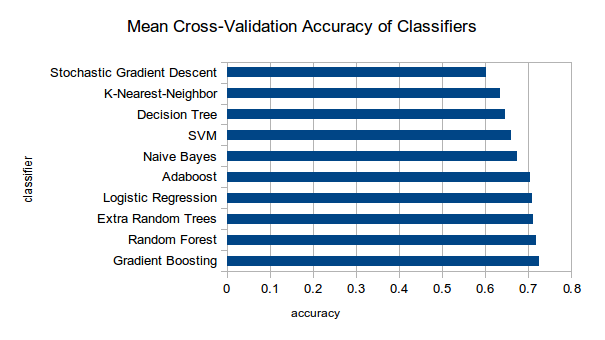
\includegraphics[width=0.75\textwidth]{crossval}
\end{figure}

\subsection{Random Forests}

Two decision-tree ensemble methods provided excellent cross-validation results and were included in our stacked classifier.
In addition to the familiar Random Forests, we also explored Extremely Random Trees.
These ensembles use random rather than discriminative thresholds when choosing features. 
They can decrease variance, but do potentially increase bias in a model.
Un-tuned on a 5-fold cross-validation of our training data, random forests achieved .7166 accuracy and extremely random trees .7112 accuracy.
Both classifiers were able to achieve .725 accuracy with parameter management. 
The main concern with these ensembles is not over-complicating them.
Helping the tree maintain their randomness helps avoid overfitting, especially when the best features are not available in a subset sample.

\subsection{Boosting}

Adaboost generates a sequence of weak, weighted classifiers which, when combined,  can provide a good model of the data.
With un-tuned parameters, Adaboost provided .7029 accuracy. It improved to approximately .72 when the model was tuned with input values.
Though often used for regression, gradient boost algorithms can be modified to perform classification.
The gradient boost algorithm performed surprisingly well in cross-validation, with .7253 accuracy.
Later optimizations of the boosting models included varying estimator quantities (e.g., 100, 200, 300, 400), varying the learning rate (e.g., 1, 0.75...) and varying the complexity of the base decision stumps.

\subsection{Logistic Regression}

Pipelining PCA to reduce the dimension of the data, followed by the logistic regression itself, showed promising performance gains.
More rigorous testing would be needed to obtain the optimal parameters. 
Without pipelining, the logistic regression algorithm performed with .7087 accuracy on 5-fold cross-validation.
Adding dimensionality reduction provided an immediate improvement, at which point the accuracy for this learner hovered around 0.72.
Regularization and penalization parameters were useful to adjust here, but basic pipelining was enough to achieve good performance (without over-complicating) in many of our tests.

\subsection{Neural Networks}

As described in Section \ref{multiple_libraries}, we wrote an adaptor class for PyBrain so that its neural network classes and functions extend the same interface as the scikit-learn Classifiers.
We used feed-forward neural networks with a back-propagation trainer.
As with the other classifiers, we imputed missing data and employed cross-validation.

The parameters for this model that we explored are the number of hidden nodes (including multiple layers) and also the number of epochs to train the Classifier for.
We primarily explored the various possibilities through the GridSearchCV function mentioned in Section \ref{tuning_parameters}.
Through this mechanism, we discovered that larger numbers of hidden nodes typically must be trained for more epochs.
However, we also found that training for too many epochs tended to overfit the training data, resulting in lower accuracy scores, especially when using cross-validation for testing.

We tried several combinations of parameters for multiple layers of hidden nodes, but did not find any that improved accuracy.
In fact, using multiple layers drastically decreased the accuracy, even when trained for a larger number of epochs.
It is possible that we simply needed to train these networks for still larger numbers of epochs, or with different amounts of hidden nodes at each layer, to realize better scores.
However, the possible combinations of parameters for multiple layers grows much faster than for a single hidden layer as the parameter space becomes a $k$-permutation of the number of nodes for $k$ layers.
Additionally, multiple hidden layer networks require more CPU cycles, and therefore real time, to train for each epoch.
Therefore, we decided to focus on a single hidden layer due to the time constraints of the project.

After identifying a reasonable number of hidden nodes to use in a network and how many epochs to train it for, we explored reducing the number of features.
We first noticed a dramatic improvement when only taking the 20 most informative features and so further explored numbers of features in the range [15,25].
The best results for number of features and model parameters are presented in Section \ref{results}.

Given more time to explore this problem, we could more fully enumerate and test different parameters.
These would include parameters that affect the learning rate and gradient steps of the neural networks.
We found that the defaults for these parameters provided by PyBrain were sufficient for our purposes and varying them would further increase the size of the parameter space to be explored.
When testing different parameters with GridSearchCV, we chose well-spaced values, such as 10, 25, 50, and 100 hidden nodes.
With more time, we could more thoroughly check these ranges to see if some values in between these might improve our classifier.

%TODO: Kyle quote about how long it takes to run deep belief networks, including with GPUs

%%%%%%%%%%%%%%%%%%%%%%%%%%%%%%%%%%%%%%%%%%%%%%%%%%%%%%%%%%%%%%%%%%%%%%

\section{Results}
\label{results}

\begin{figure}[!h]
\centering
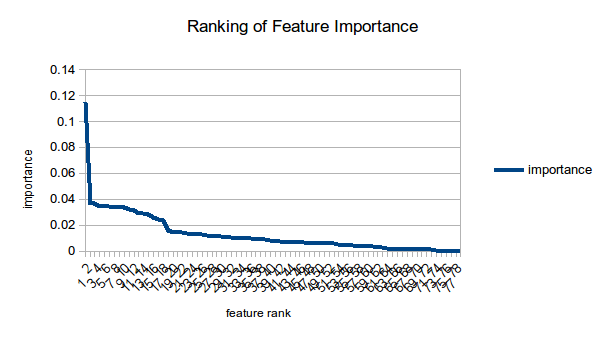
\includegraphics[width=0.45\textwidth]{feature_importance}
\end{figure}

Average 5-fold cross-validation accuracy of scikit-learn classifiers on training data (50K samples)

% 
% NN: overfit easily
% different ideal # eepochs for different # hiddens
% # features most important
% multiple layers much worse

\begin{figure}[!h]
\centering
\begin{tabular}{cc}
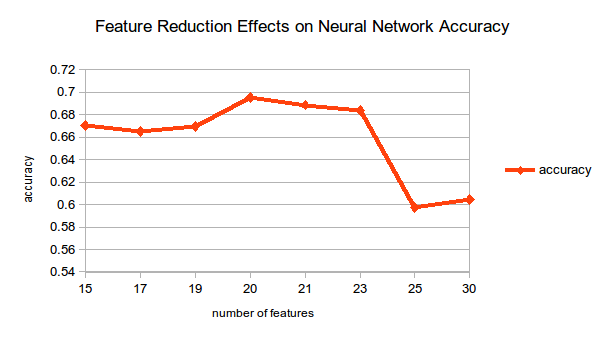
\includegraphics[width=0.45\textwidth]{nn_features} &
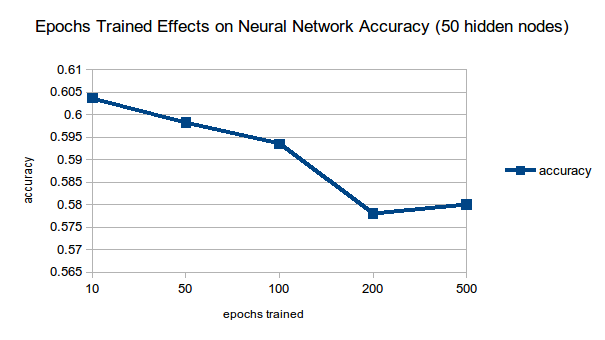
\includegraphics[width=0.45\textwidth]{nn_epochs}
\end{tabular}
\end{figure}

%%%%%%%%%%%%%%%%%%%%%%%%%%%%%%%%%%%%%%%%%%%%%%%%%%%%%%%%%%%%%%%%%%%%%%

\section{Contributions}

Eugenia implemented preprocessing functionality (imputation and feature selection) and tested 10 classifiers (without added complexity) with cross-validation on the testing data. 
After finding the 5 most powerful base classifiers (those with $> .7$ training accuracy), she added some complexity parameters and combined them into an unweighted majority-vote ensemble. 
After observing remarkable accuracy in the gradient boosting classifier for this data set, Eugenia decided to focus on its optimization.
Though she tried to optimize both for area under curve and accuracy, she found that the classifier performed better with accuracy and focused complexity updates on that metric.
She explored some academic literature concerning the 2004 KDD problems.

Kyle was curious about the potential success of a Neural Network for classification of this data, and chose its accuracy as his focus metric since it was already built into the library. 
He compared the limited neural network options available in scikit-learn with external libraries and selected PyBrain to complete his work.
He implemented a learner and added a wrapper to that it could be called with the same interface as the sci-kit learn classifiers, using GridSearchCV to quickly explore the parameter space.
Kyle also expanded on the stacked ensemble Eugenia created using the output predictions of the ``Top 5'' classifiers as input features of a logistic classifier.
This involved creating a new dataset consisting of these output predictions for each data point and running the classifier with cross-validation.
This dataset was then fed into the logistic classifier for training and another was created for the validation dataset to record the final predictions.


%%%%%%%%%%%%%%%%%%%%%%%%%%%%%%%%%%%%%%%%%%%%%%%%%%%%%%%%%%%%%%%%%%%%%%

\section{Conclusion}

TODO Comment on our findings, surprises, etc.
such as ensemble doing worse than individual learners

In many real-world machine learning tasks, time and hardware constraints can limit the feasibility of fully exploring the problem space.
In order to succeed in this project, we had no choice but to specialize classifiers, features, testing strategies, and ensemble combination approaches.
Reflecting on the experience, we would be particularly interested on optimizing for a custom metric (such as SLQ) in the future.
Some challenges of non-traditional metric evaluation are commented on in \cite{vogel2004anti}.
Caruana notes in their overview of the KDD 2004 competition field \cite{caruana2004kdd} that optimizing for one parameter and submitting the data for comparison to another (e.g., accuracy optimized, then submitted to cross-entropy) yielded poor performance on the latter metric. 
The SLQ metric is captivating because it is specific to the particle physics problem and its stakeholder research communities. 

Our workflow for selecting and combining configurations of ensemble classifiers has helped us understand how to most effectively approach complex machine learning problems in our future research endeavours.
In particular, the use of automated functions for exploring parameter spaces in parallel proved quite effective in finding model parameters that produced high accuracy predictions.
In the future, we intend to further automate this process by having the functions themselves determine which parameter values to try, rather than our approach of manually choosing spreads of values that was necessary due to very limited time and computational resources.

%%%%%%%%%%%%%%%%%%%%%%%%%%%%%%%%%%%%%%%%%%%%%%%%%%%%%%%%%%%%%%%%%%%%%%

\bibliographystyle{IEEEtran}
\bibliography{report}

\end{document}
